\chapter{Results}
\label{chapter:results}

% \begin{figure}[b]
    \vspace{-0.7cm}
      \centering
      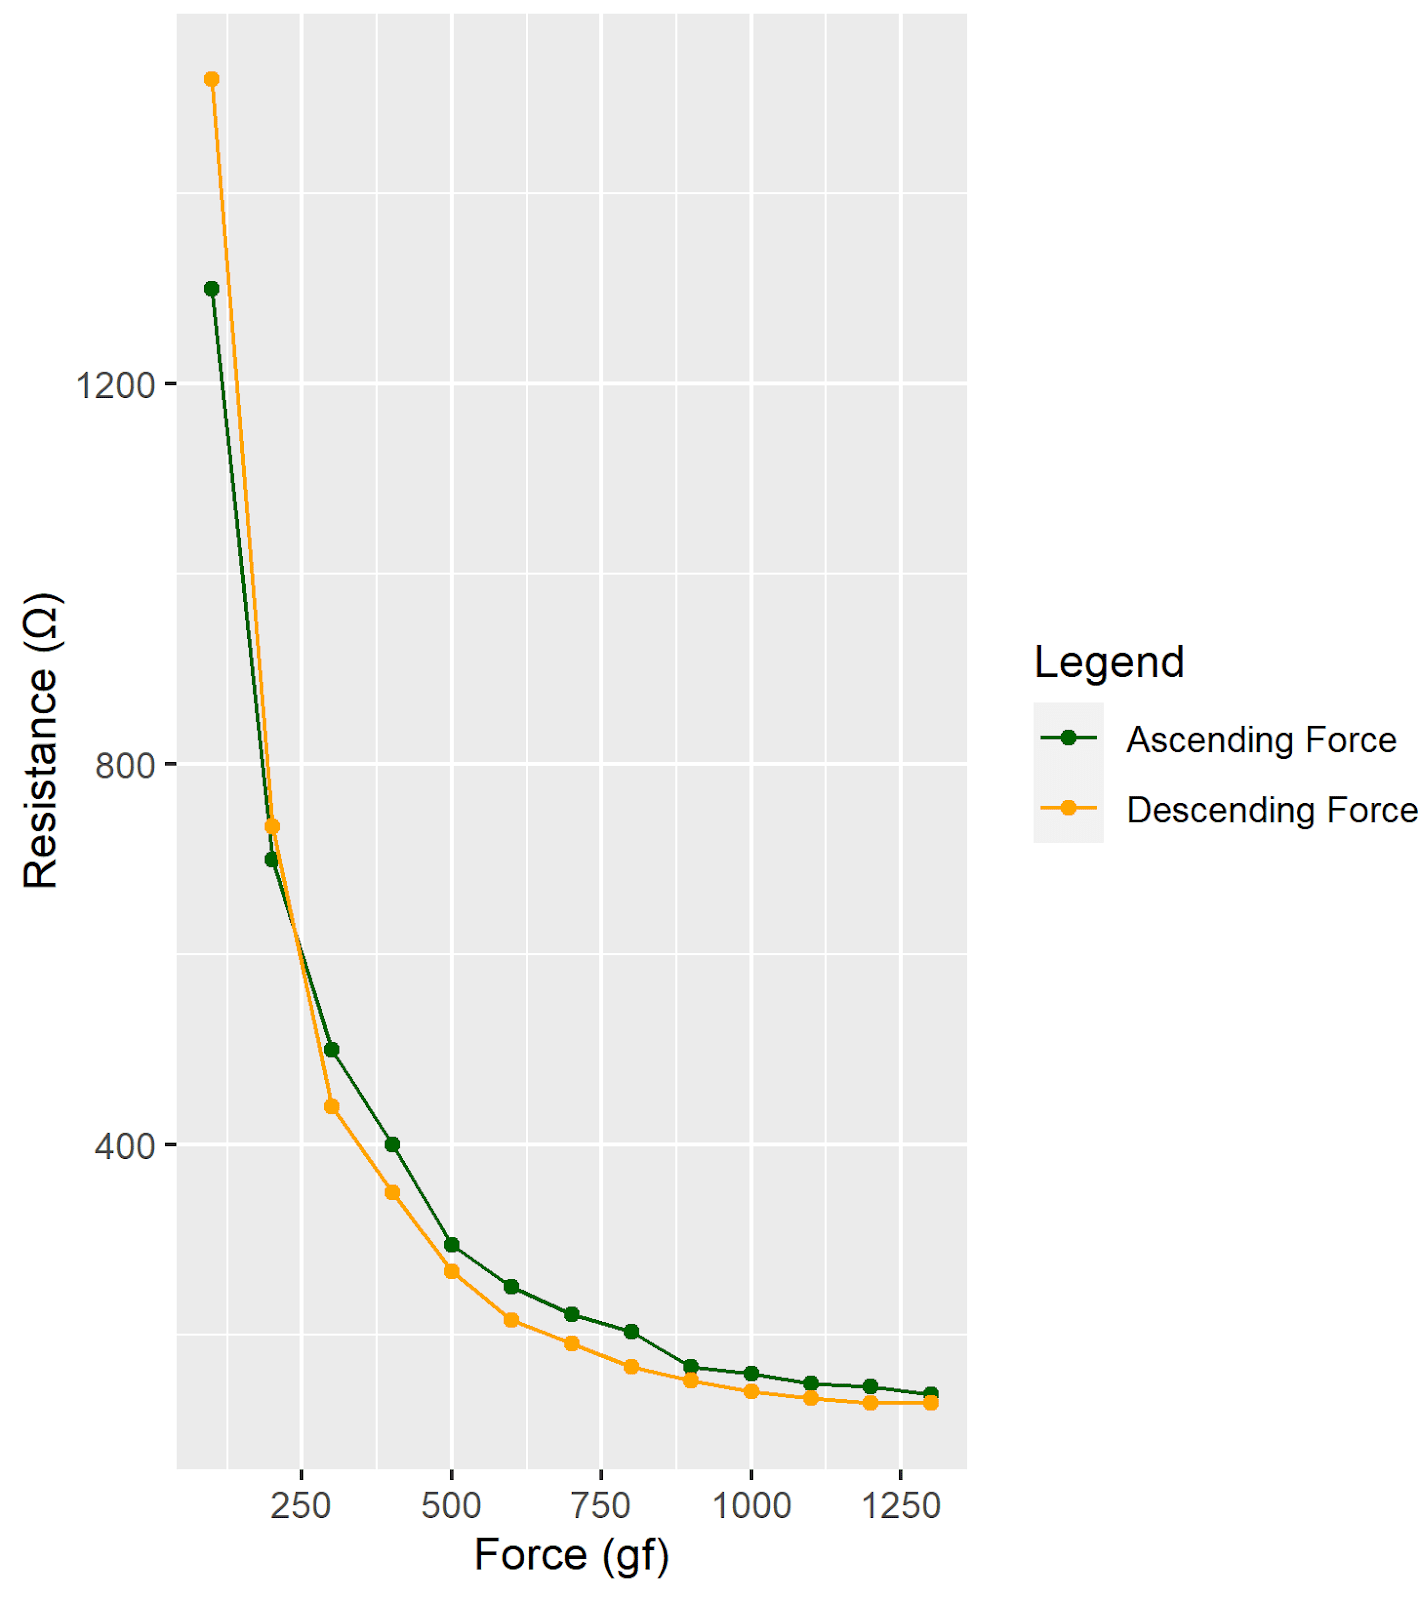
\includegraphics[width=0.5\textwidth]{figs/ascending_descending.png}
      \vspace{-0.2cm}
      \caption[Resistance vs Pressure Relationship]{Resistance vs Pressure Relationship for Velostat}
      \label{fig:velostat}
\vspace{1.0cm}
\end{figure}

% The relation between the pressure and resistance was non-linear as we expected.

% \begin{figure}
    \centering
    \begin{subfigure}[b]{0.4\textwidth}
        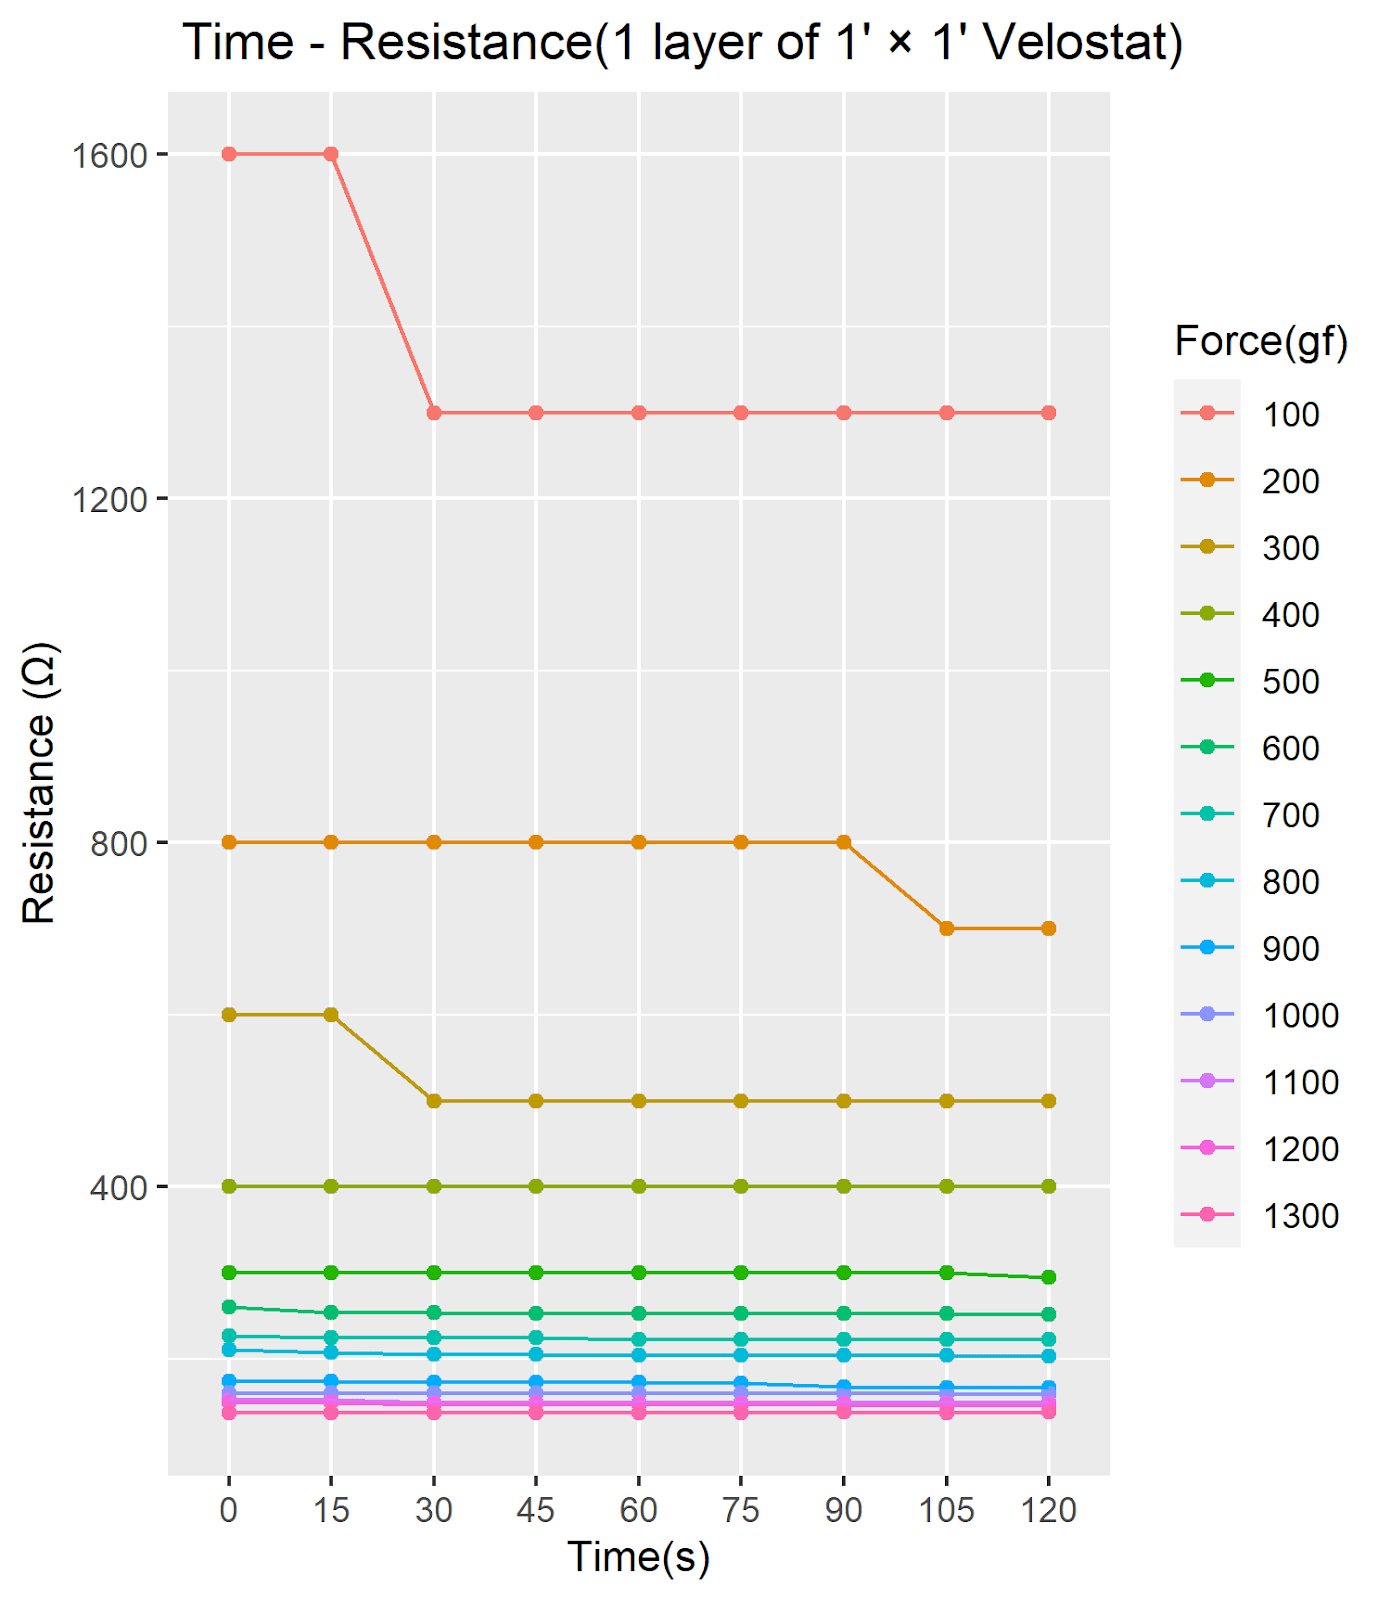
\includegraphics[width=\textwidth]{figs/one_layer.png}
        \caption{One layer of Velostat}
        \label{fig:one_layer}
    \end{subfigure}
    ~ %add desired spacing between images, e. g. ~, \quad, \qquad, \hfill etc. 
      %(or a blank line to force the subfigure onto a new line)
    \begin{subfigure}[b]{0.4\textwidth}
        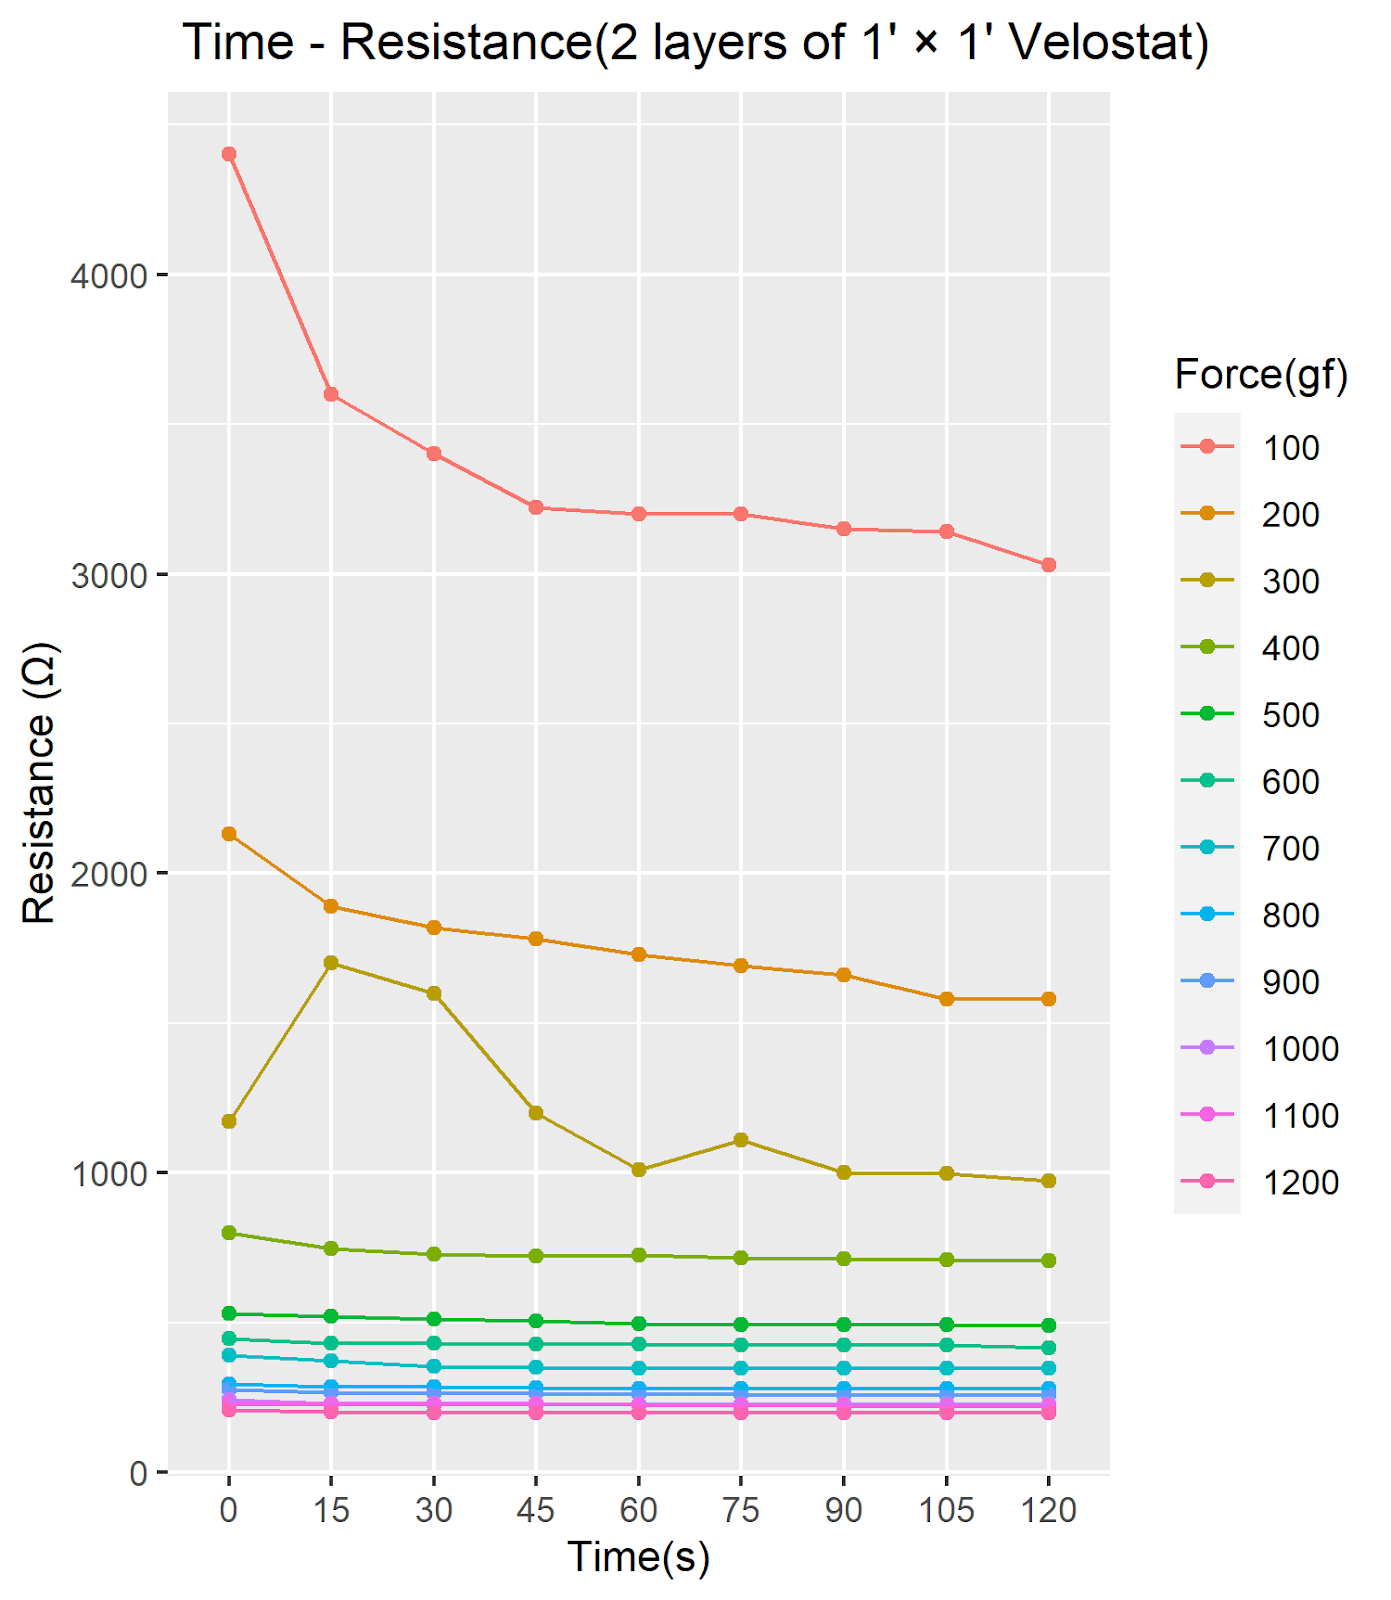
\includegraphics[width=\textwidth]{figs/two_layer.png}
        \caption{Two layers of Velostat}
        \label{fig:two_layer}
    \end{subfigure}
    \hfill %add desired spacing between images, e. g. ~, \quad, \qquad, \hfill etc. 
    %(or a blank line to force the subfigure onto a new line)
    \vspace{0.2cm}
    \caption[Compare No. of Layers]{Time for stable resistance value was higher in the case of two layers than one layer}\label{fig:hysterisis}
\end{figure}

 

% The pressure mat frames are mapped with color scheme Jet and Gaussian interpolation is used to get the final output. Since there was huge difficulties for a proper and careful calibration in the overall pressure mat we could not get highly satisfactory results. But the mat detected areas corresponding to high pressure approximately. More statisfactory image was obtained for feet when standing on the mattress. \begin{figure*}
    \vspace{-0.7cm}
      \centering
      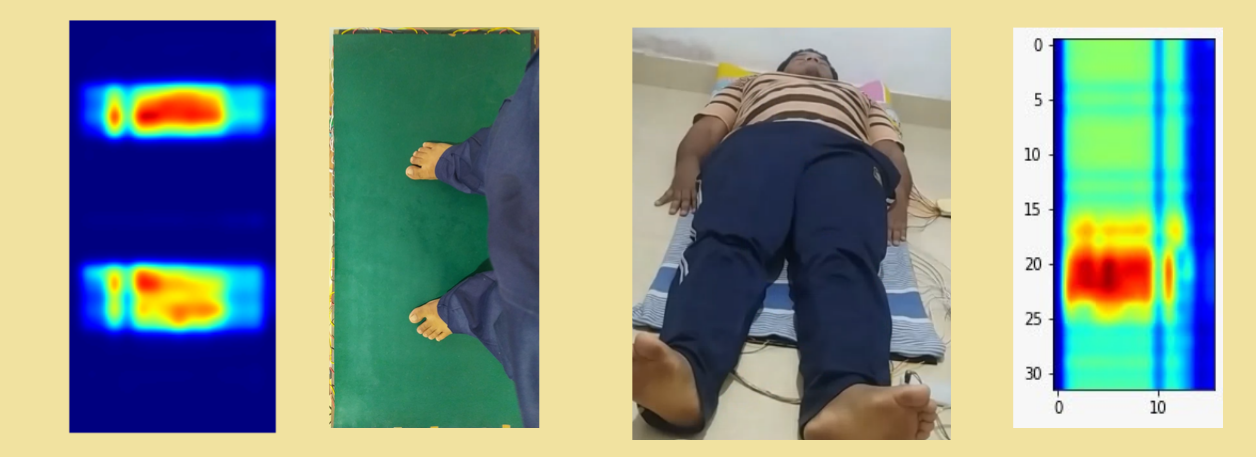
\includegraphics[width=\textwidth]{figs/mat_frames.png}
      \vspace{-0.2cm}
      \caption[Mat frames]{Pressure mat frames}
      \label{fig:mat_frames}
\vspace{1.0cm}
\end{figure*}

% Several 1.2kg discs were used to check parts of the mattress.

% When an pressure image is sent to the server end point and the posture is detected. Then there are particular ulceration points that are active for that posture. Providing the pressure image and these ulceration point names as the input bounding box parameters can be obtained.
% \begin{figure*}[t]
    \vspace{-0.7cm}
      \centering
      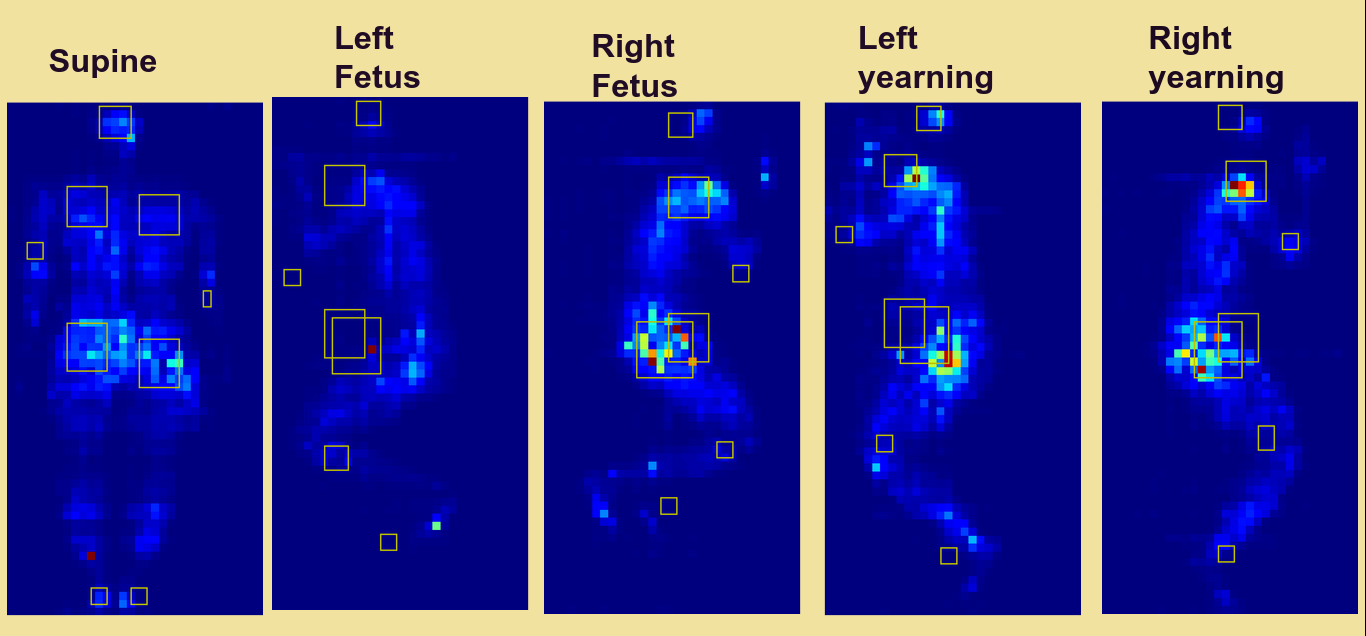
\includegraphics[width=\textwidth]{figs/ml_result.png}
      \vspace{-0.2cm}
      \caption[Results from Neural Network Models]{Results from Neural Network Models}
      \label{fig:mlresult}
\vspace{1.0cm}
\end{figure*}
% All five postures classified correctly and bounding boxes are marked appropriately as in the figures.

% When ulceration points are located the pressure of these points can be found. We simulated temporal behavour and repositioning using the dataset by University of Dallas.

% Repositioning considerably shifts the pressure distribution. 

% \begin{figure*}
    \vspace{-0.7cm}
      \centering
      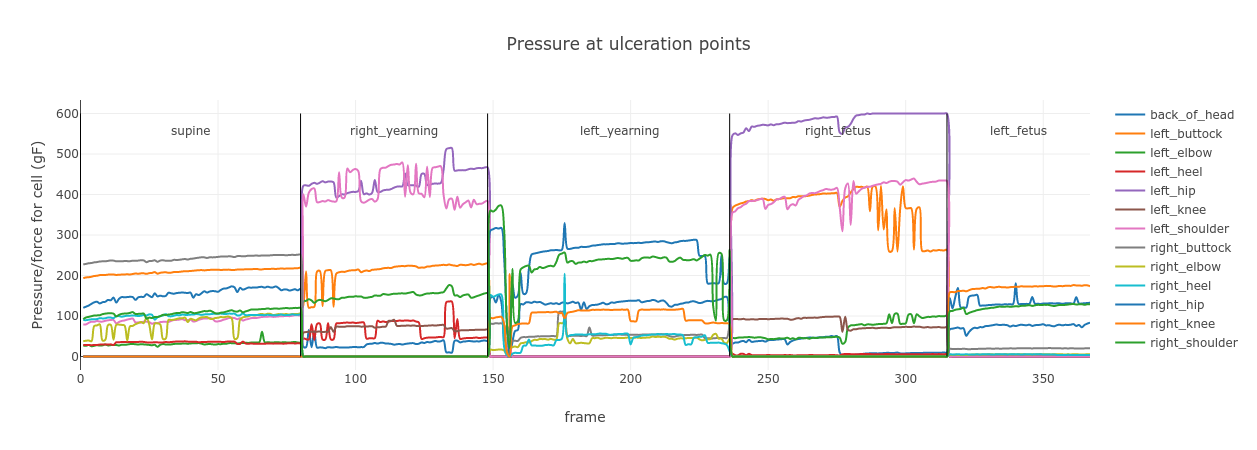
\includegraphics[width=\textwidth]{figs/simulation.png}
      \vspace{-0.2cm}
      \caption[Simulation]{Simulation.}
      \label{fig:simulation}
\vspace{1.0cm}
\end{figure*}




The relationship between resistance and pressure is non-linear (as expected for Velostat).\begin{figure}[b]
    \vspace{-0.7cm}
      \centering
      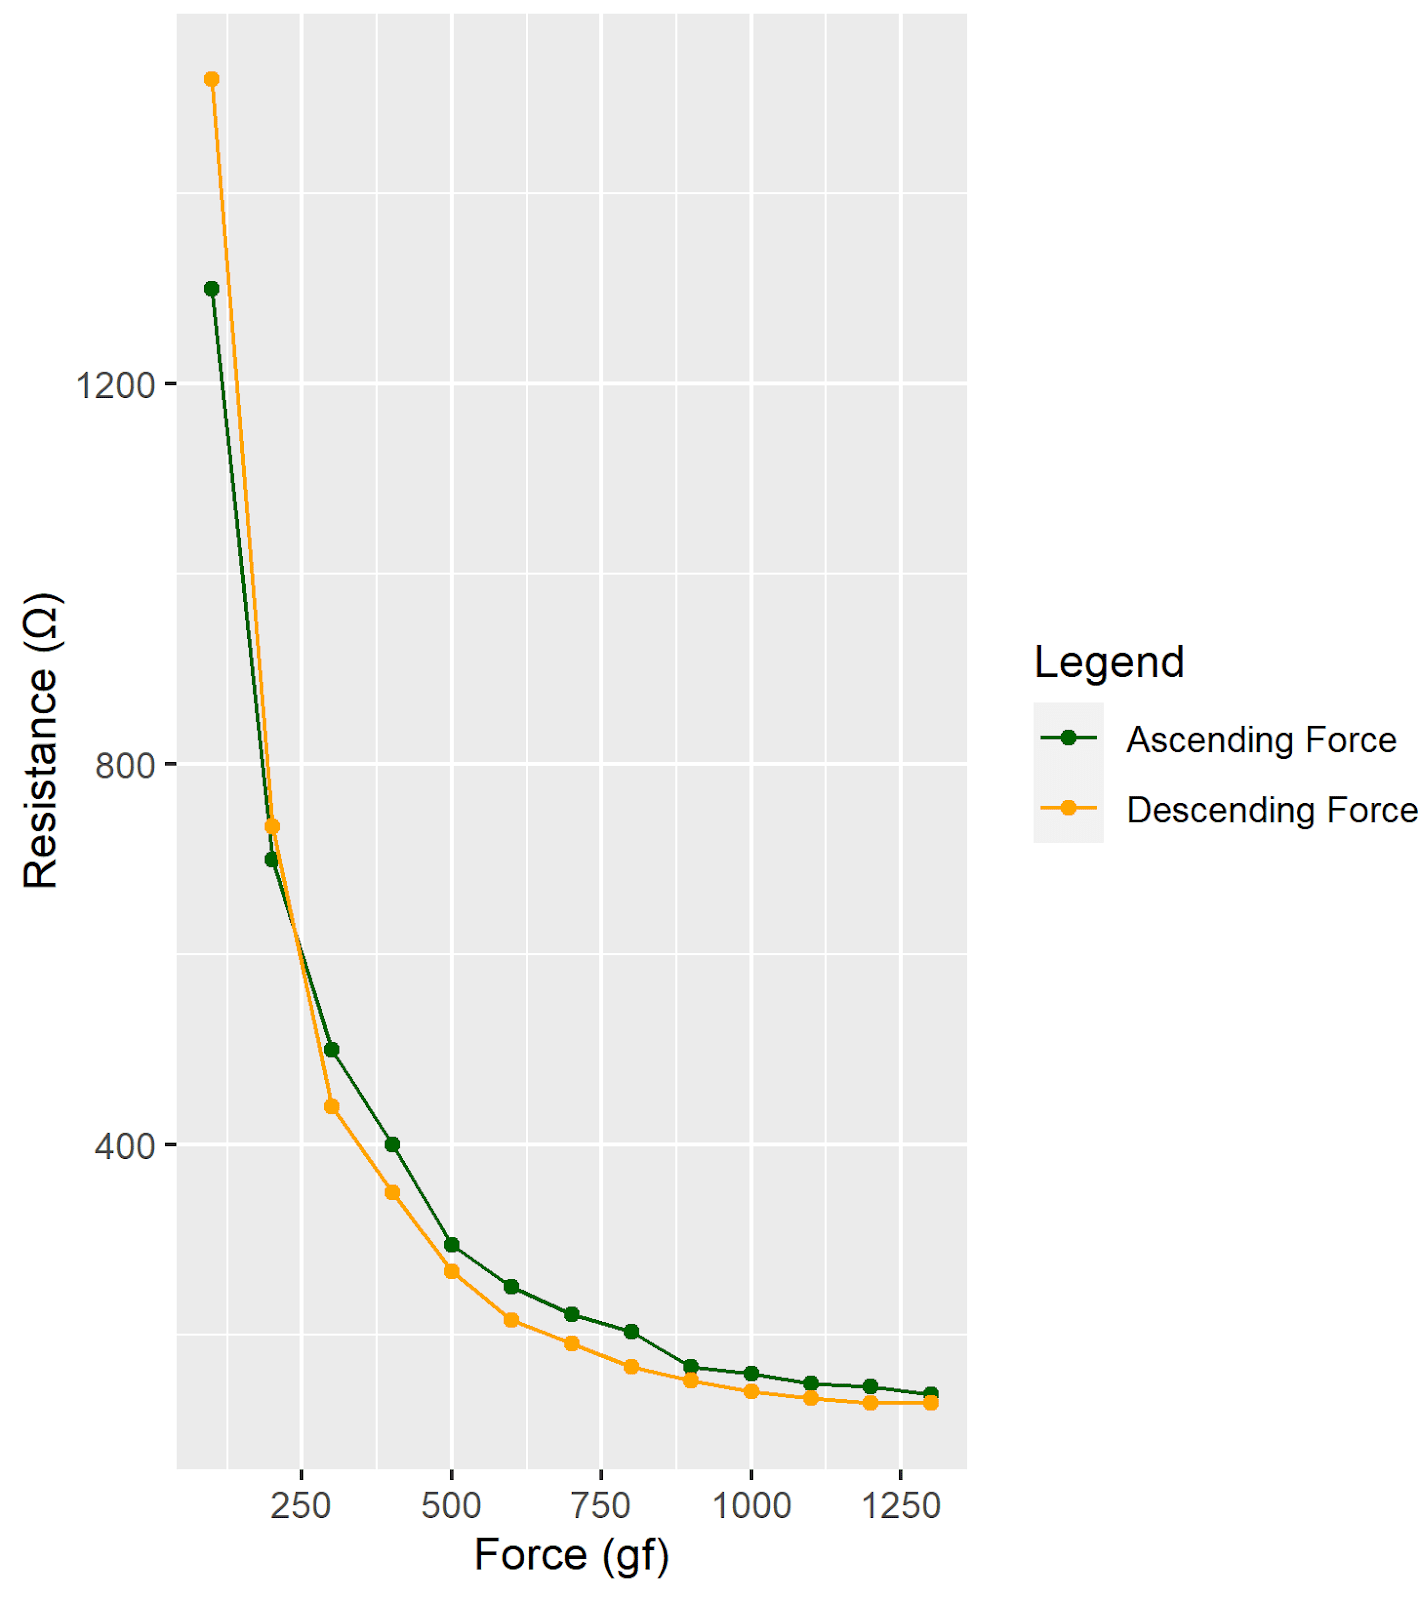
\includegraphics[width=0.5\textwidth]{figs/ascending_descending.png}
      \vspace{-0.2cm}
      \caption[Resistance vs Pressure Relationship]{Resistance vs Pressure Relationship for Velostat}
      \label{fig:velostat}
\vspace{1.0cm}
\end{figure} Comparing the curves under ascending and descending forces it can be seen that hysterisis effects are tolerable. Comparing two layers of Velostat against one layer it was revealed that although the sensitivity improved the time for a stable result higher in the case of two layers. Therefore one layer of Velostat is appropriate for the pressure mats. \begin{figure}
    \centering
    \begin{subfigure}[b]{0.4\textwidth}
        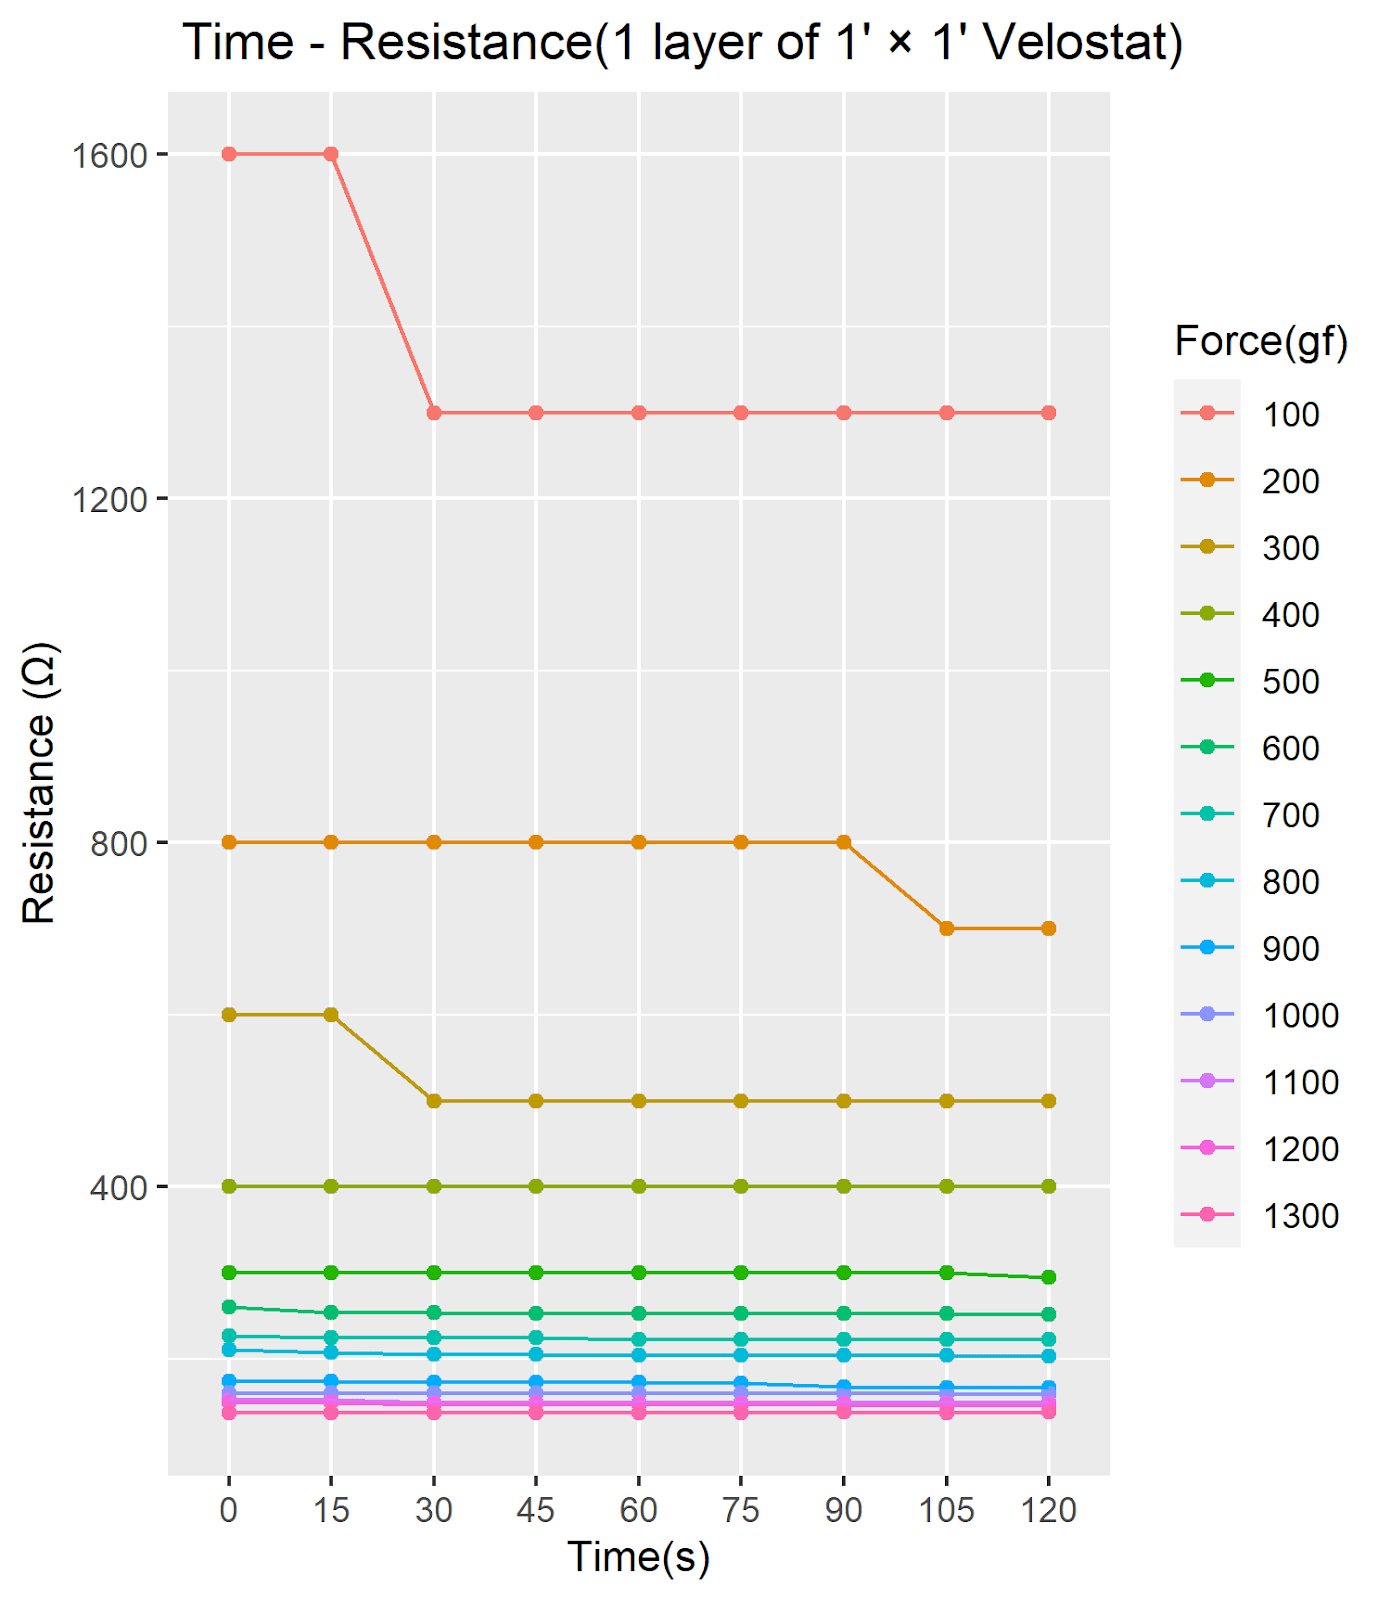
\includegraphics[width=\textwidth]{figs/one_layer.png}
        \caption{One layer of Velostat}
        \label{fig:one_layer}
    \end{subfigure}
    ~ %add desired spacing between images, e. g. ~, \quad, \qquad, \hfill etc. 
      %(or a blank line to force the subfigure onto a new line)
    \begin{subfigure}[b]{0.4\textwidth}
        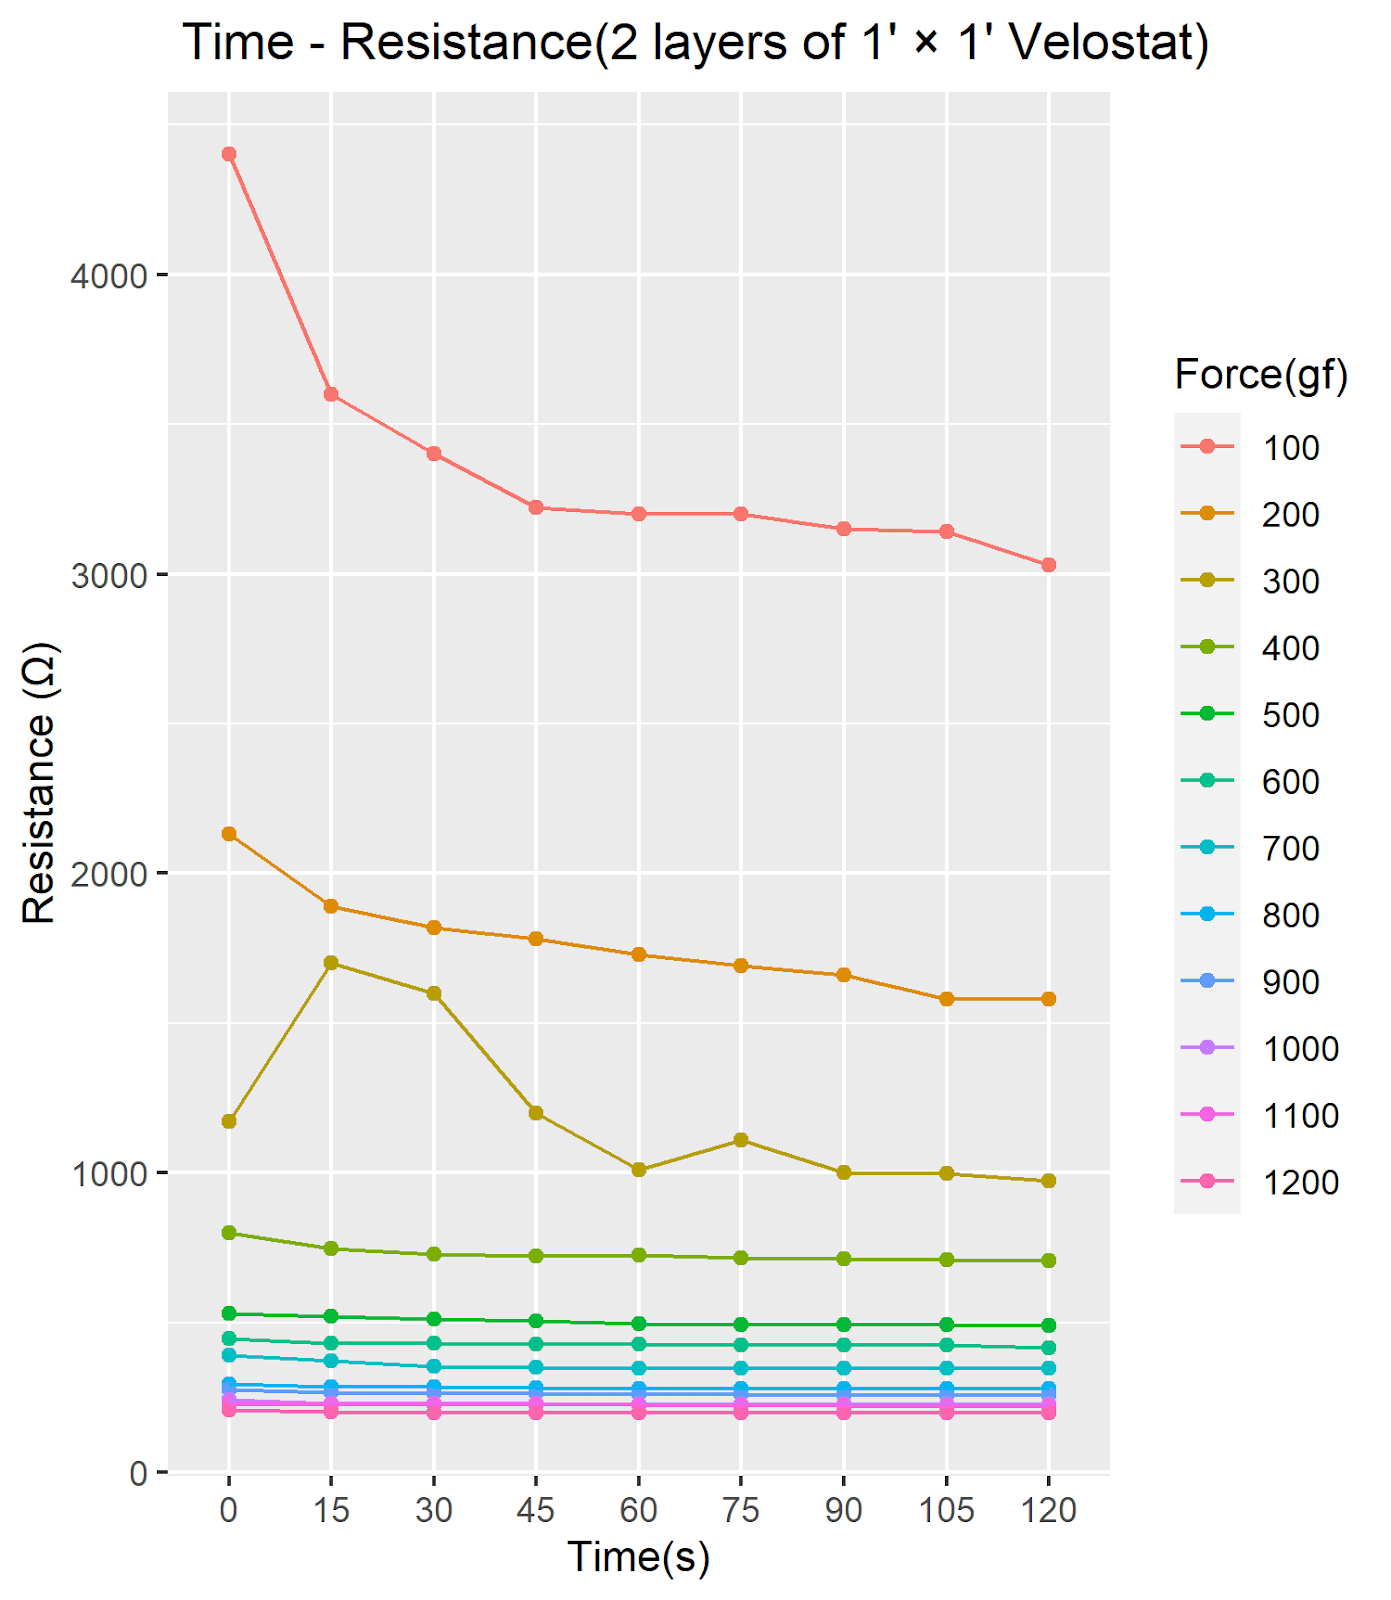
\includegraphics[width=\textwidth]{figs/two_layer.png}
        \caption{Two layers of Velostat}
        \label{fig:two_layer}
    \end{subfigure}
    \hfill %add desired spacing between images, e. g. ~, \quad, \qquad, \hfill etc. 
    %(or a blank line to force the subfigure onto a new line)
    \vspace{0.2cm}
    \caption[Compare No. of Layers]{Time for stable resistance value was higher in the case of two layers than one layer}\label{fig:hysterisis}
\end{figure}


\section{Frames of Pressure Mat Readings}
The frames from pressure mat are mapped with color scheme Jet and Gaussian interpolation is used to get the final output. Since there was huge difficulties for a proper and careful calibration in the overall pressure mat we could not get highly satisfactory results. But the mat detected areas corresponding to high pressure approximately. More statisfactory image was obtained for feet when standing on the mattress. Several 1.2kg discs were used to calibrate parts of the mattress. \begin{figure*}
    \vspace{-0.7cm}
      \centering
      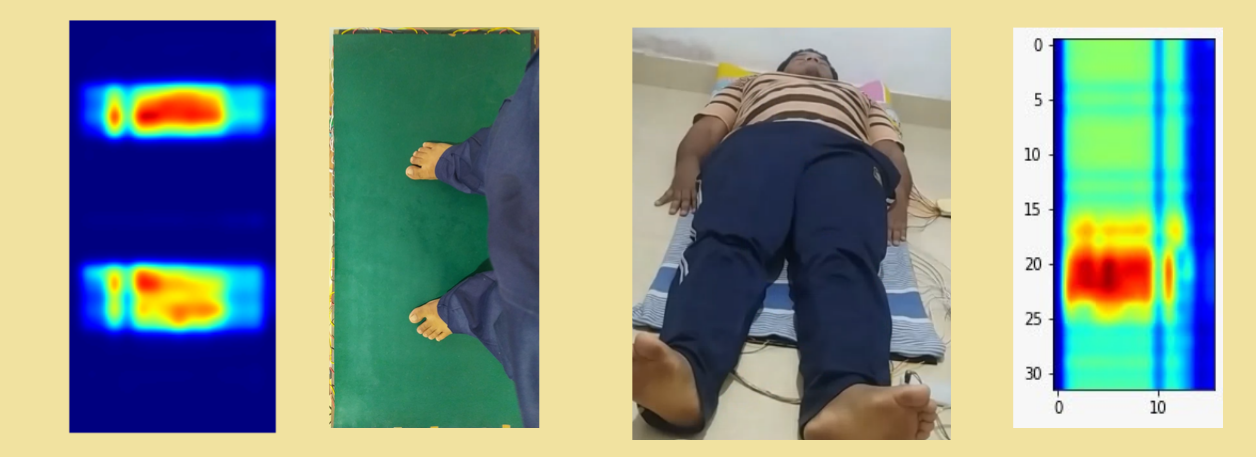
\includegraphics[width=\textwidth]{figs/mat_frames.png}
      \vspace{-0.2cm}
      \caption[Mat frames]{Pressure mat frames}
      \label{fig:mat_frames}
\vspace{1.0cm}
\end{figure*}

\section{Neural Network results}
When a pressure image is sent to the server end point the posture is detected by the posture detection model. Then there are particular ulceration points that are active for that posture. Providing the pressure image and these ulceration point names as the input, bounding box parameters can be obtained.
All five postures classified correctly and bounding boxes are marked appropriately as in the figures.\begin{figure*}[t]
    \vspace{-0.7cm}
      \centering
      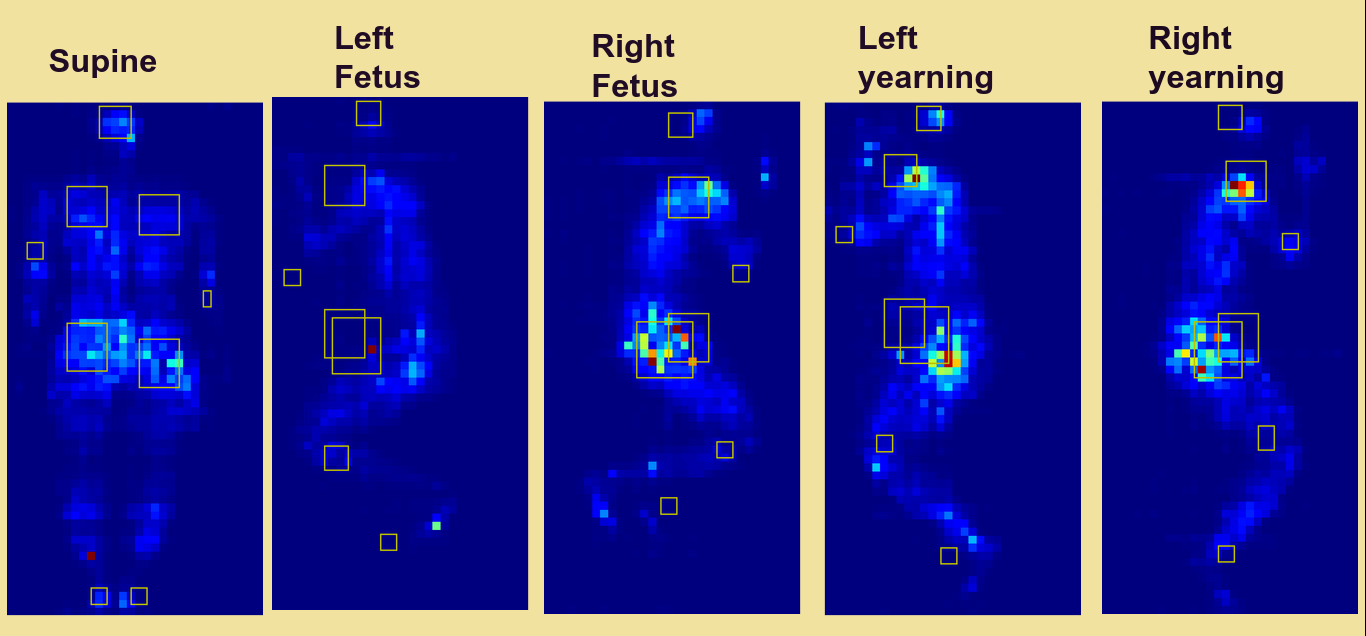
\includegraphics[width=\textwidth]{figs/ml_result.png}
      \vspace{-0.2cm}
      \caption[Results from Neural Network Models]{Results from Neural Network Models}
      \label{fig:mlresult}
\vspace{1.0cm}
\end{figure*}

\section{Simulation of pressure-time behaviour on ulceration points}

When ulceration points are located the pressure of these points can be found. We simulated temporal behavour and repositioning using the dataset by University of Dallas.Repositioning considerably shifts the pressure distribution and the pressure values are almost stable in a particular posture.

\begin{figure*}
    \vspace{-0.7cm}
      \centering
      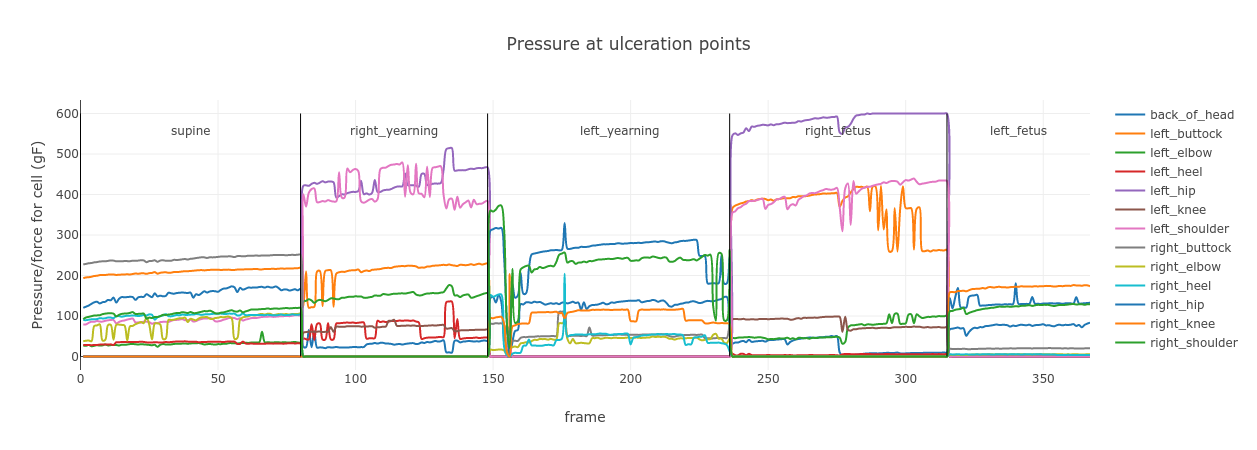
\includegraphics[width=\textwidth]{figs/simulation.png}
      \vspace{-0.2cm}
      \caption[Simulation]{Simulation.}
      \label{fig:simulation}
\vspace{1.0cm}
\end{figure*}

\section{Implementation}

\begin{description}
    \item[The information system]   \url{http://prevelcer.herokuapp.com}
    \item[App] React native based app
    \item[API documentation] \url{https://documenter.getpostman.com/view/13647586/TVmHDeox}
    \item[Neural Network Models] \url{http://prevelcernn.herokuapp.com}
\end{description}




